% Chapter Template

\chapter{FM-Index} % Main chapter title

\label{Chapter2} % Change X to a consecutive number; for referencing this chapter elsewhere, use \ref{ChapterX}

%----------------------------------------------------------------------------------------
%	SECTION 1
%----------------------------------------------------------------------------------------
%\begin{figure*}[h]

%	\vspace*{-60mm}
%	\hspace*{60mm}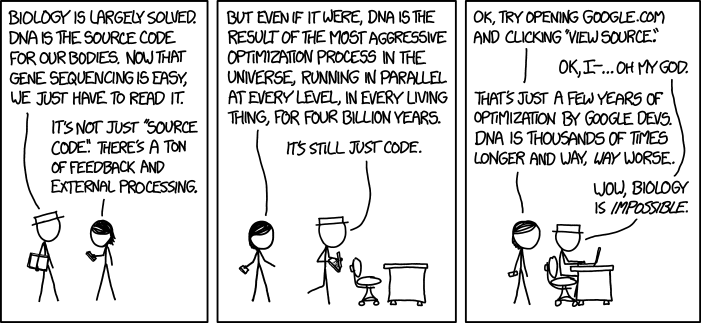
\includegraphics[scale = 0.3]{Figures/xkcd.png}
%\end{figure*}
%\vspace*{15mm}

With the observations afore stated about the nature and form of the data in the context of genomics, it seems obvious that an appropriate data structure for those, along with an efficient algorithm, might to a serious gain in performance in the short reads alignments. The \textsl{FM-Index} is a lossless compression algorithm based on the \textsl{Burrows-Wheeler Transform} that offers such gains by reorganizing the data in a way that may reduce both memory needs and latency of the mapping process. 

Both those concepts are the subject of the next sections, followed by a \textsl{Python} implementation, which aims to better illustrate the whole read alignment process, and a \textsl{C++} implementation of the same algorithm which will be then used for the hardware implementation.

\section{Theoretical Concepts}

Introduced by \textsl{Michael Burrows} and \textsl{David Wheeler} in 1994, the \textsl{Burrows-Wheeler Transform} (BWT) rearranges the characters of a \textit{string} into sequences of similar characters by a series linear operations. Although it does not reduce the size of the input data, the rearrangement thus obtained gets greatly improved compression results. Furthermore, the easy reversibility of the process substantially facilitate data manipulation employed in sequence alignment, such as finding the original position from the determined one in the transform. This process is further detailed in the next section.

\subsection{Burrows-Wheeler Transform Algorithm}

The transform can be divided in 4 main steps\footcite{BWT0} :
\begin{enumerate}
\item Append a special character (usually represented as a \$), lexicographically smaller than any others, at the end of the input string \textrm{T}.
\item Construct a square matrix $M_T$ with each being another iteration of a left rotating shift applied to the original string.
\item Sort $M_T$ in lexicographical order
\item Get the transformed text output $T^{bwt}$ by selecting the last column of $M_T$ 
\end{enumerate}

\begin{figure}[h]
\centering
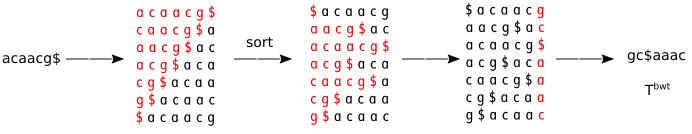
\includegraphics[scale=0.65]{Figures/bwt.png}
\caption{Illustration of the \textsl{BWT} applied to the string \textit{acaacg}}
 \label{fig:bwt}
 \end{figure}
The figure \ref{fig:bwt} above illustrates the process of the \textsl{BWT}, it will be shown next what is used in the mapping process, but first let us note the following properties :
\begin{enumerate}
\item the process is revertible as it consists exclusively of linear operations
\item all columns are permutations of the input $T$
\item the last columns contains mostly all similar character consecutively
\item the first column contains all characters in lexicographical order, so the first row will always start with the inserted \$ symbol (i. e. be the first rotation applied to $T$)
\item Occurrences of a character $c$ in the first column are sorted the same way than in the last column, meaning ranks order in the first and last column match, as depicted in figure \ref{fig:LF}
\end{enumerate}



From a compression perspective, the $T^{bwt}$ result is a way better candidate than its original form as it sees most of similar characters regrouped, hence allowing shorter encoding for those sequences\footnote{http://www.hpl.hp.com/techreports/Compaq-DEC/SRC-RR-124.pdf}. Furthermore, properties 1, 2 and 5 indicate an easy transition, if needed, back to the original text  using the  \textsl{LF Mapping} illustrated in figure \ref{fig:LF} and formally defined in equation \ref{eq:LF}. \\

For $Occ$ an array containing, for each symbol $c$ of the alphabet $\Sigma$, the index of its first occurence in the first column $F$ and $Count(i, c)$, a function returning the number of occurences of $c$ in $F$ at given index $i$, we can define the $Last-to-First$ mapping as follow :
\begin{equation}
    LF(i, c) = Occ[c] + Count(i, c)
    \label{eq:LF}
\end{equation}


\begin{minipage}[t]{0.5\textwidth}
    \begin{figure}[H]
\hspace{-15mm}  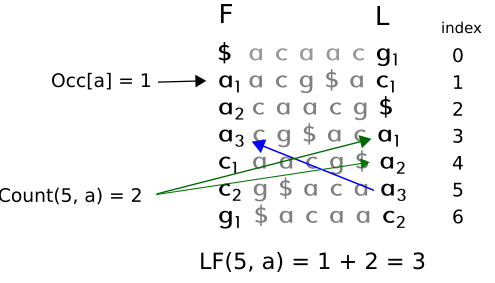
\includegraphics[scale = 0.5]{Figures/LF.png}
  \caption{LF-Mapping of $3^{rd}$ occurrence of $a$ from last column}
    \label{fig:LF}
\end{figure}
\end{minipage}
\begin{minipage}[t]{0.4\textwidth}
        This figure illustrates how the mapping is done : from the fact that character ranking are the same in both last and first column (and all the others for that matter), the \textsl{LF-Mapping} algorithm enables retrieval of the position in $F$ for any character in $L$. This method is used in the \textsl{Walk-Left} algorithm to reconstruct the original text, which is thereafter further detailed in figure \ref{fig:walkleft}.
\end{minipage}
\vspace*{5mm}

Finally, from a search point of view, the last property is the most interesting. Lexicographical order allows for spatial proximity of sought result, hence, an iterative search through a word to find in $T^{bwt}$ will see each iteration to indicate spatially close positions which yet facilitates this process.\\

Now that this concept is well defined, the next section will aim to illustrate how the FM-Index algorithm makes the best out of this transform in order to enable efficient data compression and sub-string queries.

\subsection{FM-Index}

An \textsl{FM-Index} is a lossless text compression based on the \textsl{BWT}\footcite{FM_INDEX}, it was created by \textsl{Paolo Ferragina} and \textsl{Giovanni Manzini} whom refer to it as an \textit{"opportunistic data structure"}. The design of this index is based upon the combination of the BWT and the suffix array data structure, displayed in red in figure \ref{fig:bwt}.\footnote{https://pdfs.semanticscholar.org/d896/e62b6cbfd623d1d9041f90b7f9e41d1451a7.pdf}

\paragraph{Creating an FM-Index}

In order to create the \textsl{FM-Index} of an input full-text \textit{string} $T$, one must create its \textsl{BWT} transform $T^{bwt}$ as explained in the previous section. Referring again to figure \ref{fig:bwt}, the \textcolor{red}{red} sub-matrix from the one in the middle, i.e. the suffix array (SA) will also be used. Finally, the index itself, noted $F$ will be constructed from the SA and $T^{bwt}$.

So, for a given $T^{bwt}$ of $N$ symbols and an alphabet $\Sigma$ of $\sigma$ elements, we define the FM-Index $F$ as a two-dimensional matrix with $(N + 1)$ rows and $\sigma$ column. For a given index $i$ (row) and a given symbol $c$ (column), $F[i][c]$ contains the number of occurrences of $c$ before the index $i$ in $T^{BWT}$. From this definition, we can construct the whole index for $T^{bwt}$, initializing $F[0]$ at $0$ and $\forall$ $i$ from $0$ to $N$, copy $F[i]$ into $F[i+1]$, incrementing $F[i+1][c]$ only if $T^{BWT}[i]$ = $c$. The last entry $F[N + 1]$ represents the total number of occurrences of all symbols in $T^{bwt}$. Using this index, we can statically compute the $Occ$ array of length $\sigma$, which stores the index of the first suffix starting with each symbol in the suffix array.

\paragraph{LF-Mapping, Walk-Left and String Matching Algorithms}
We now have all the elements required to describe the LF-Mapping function for $i$ the current index and $c \in \Sigma$ the queried symbol in $T^{bwt}$  : 
\begin{equation*}
LF(i, c) = Occ[c] + F[i][c]
\end{equation*}
The return value is the index of the corresponding character in the suffix array. \\
Using this function, we can define the \textsl{Walk-Left} algorithm to invert the BWT and retrieve to original string $T$. \\

\begin{minipage}[t]{0.55\textwidth}
\begin{algorithm}[H]
	\SetAlgoLined
	\KwIn{BWT $T^{bwt}$, FM-Index $F$, First occurrences $Occ$, index $i$}
	\KwOut{The original input strinp $T$}
	i = 0\;
	t = ""\;
	\While{$T^{bwt}[i] \neq $ "\$"}{
		t = $T^{BWT}[i] $ + t\;
		i = $LF(i, T^{BWT}[i])$\;
	}
\caption{Walk-Left - Inverting the BWT}
\end{algorithm}
\end{minipage}
\hspace{3mm}
\begin{minipage}[t]{0.3\textwidth}
Blablablabla blabla bla bla bla bla bla
\end{minipage}
\vspace*{5mm}

\begin{figure}[H]
\centering
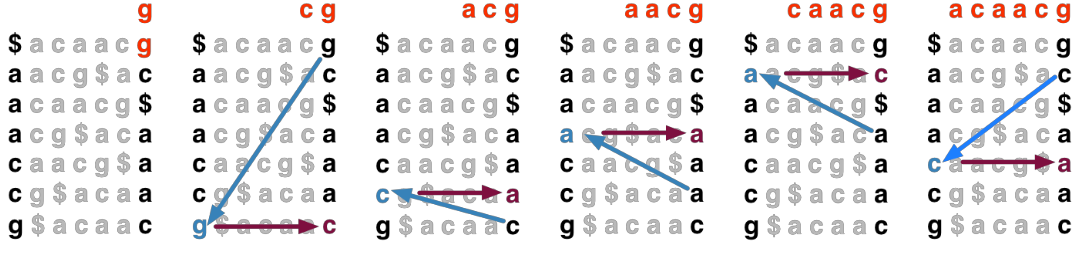
\includegraphics[scale = 0.4]{Figures/WL_algo.png}
\caption{Illustration of the Walk-Left Algorithm inverting the $T^{bwt}$ to retrieve original text $T$}
\label{fig:walkleft}
\end{figure}

Using the same function, we now define an algorithm that, given a BWT $T^{bwt}$ and a query string $q$, will return the index range in the implicit suffix array containing $q$ : \\

\begin{minipage}[t]{0.55\textwidth}
\begin{algorithm}[H]
\SetAlgoLined
\KwIn{BWT $T^{bwt}$, FM-Index $F$, First occurrences $Occ$, query string $q$}
\KwOut{Index Range $top$, $bot$ for $q$ in the suffix array corresponding to $T^{bwt}$ }
	$top$ = 0\;
	$bot$ = $len(T^{BWT})$\;
	\For{$qc$ in $reverse(q)$}{
		$top$ = $LF(top, qc)$\;
		$bot$ = $LF(bot, qc)$\;
}
\caption{Exact String Matching in Suffix Array}
\end{algorithm}
\end{minipage}
\hspace{3mm}
\begin{minipage}[t]{0.3\textwidth}
Blablablabla blabla bla bla bla bla bla
\end{minipage}

\begin{figure}[H]
\centering
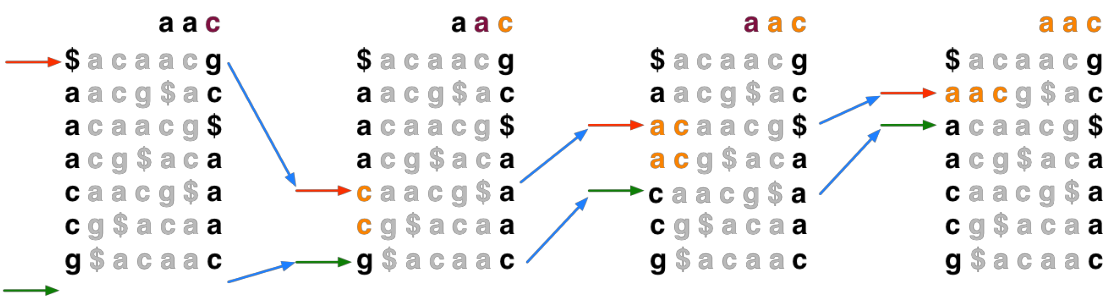
\includegraphics[scale = 0.35]{Figures/matching_algo.png}
\caption{Illustration of the matching process of the string  $q$ = $"aac"$ in the suffix array derived from $T^{bwt}$ }
\end{figure}


If the return range $[top, bot]$ is empty, then the queried string $q$ does not appear in the reference text.


\paragraph{Putting it all Together}

Now that all the data structures and computational tools have been introduced, we can define the process of exact string matching using the FM-Index, in an input reference string $T$ and a string query $q$ :
\begin{enumerate}
\item Compute the Burrows-Wheeler Transform $T^{bwt}$ of $T$, use it to find $Occ$ and to get the FM-Index $F$.
\item Use Algorithm 2 to determine the index of the rotation in the implicit suffix array containing $q$
\item If such an index exists (i.e. $q$ occurs at least once in $T$), use the Walk-Left Algorithm to walk back to the beginning of the text from this index
\item The number of steps corresponds to the offset of $q$ in $T$
\end{enumerate}

\paragraph{Performance Analysis}

As mentioned earlier in this document, the size of a genomic dataset is usually in the billion of entry range. Hence, we consider the following items in the previously defined process to be way too costly time or space-wise : 
\begin{itemize}
	\item Step 4 of the procedure requires a number of step linear to the length of $T$. Doing this may require billions of iterations over the lines $4$ and $5$ of Algorithm 1, meaning billions of memory access, which is way too much time consuming.
	\item Storing the whole FM-Index requires storing $(N + 1)*\sigma$ values, with $N$ the length of $T$ and $\sigma$ the size of its alphabet $\Sigma$. This would require in our case at least 6 times the size of $T$ in memory space, which is way too big.
	\end{itemize}
	In order to reduce both those costs, the following solution is introduced :
	\begin{itemize}
		\item Keep samples of the suffix array index (e.g. every 32$^{th}$ row), when "walking" back along $T^{BWT}$ check if an entry exists for the current position, if yes, then add this value to the number of step already done to obtain the position of $q$ in $T$. This allows to Walk-Left algorithm to operate in a constant time, while limiting the space needed to store those values.
		\item Keep only some samples of the FM-Index (e.g. one every 128 entries), referred as " checkpoints ". The LF function would now take the index of the current symbol in $T^{bwt}$ and find the closest surrounding checkpoint, then "walk" along $T^{bwt}$, counting the occurrences of the same symbol along the way and adding/subtracting (respectively if the closest checkpoint is above or below the current index) this count to the rank value stored in the checkpoint. This reduces greatly the space needed to store the index, while keeping a constant computation time for the LF function.
		\end{itemize}
		
		\begin{figure}[h]
			\centering
			\begin{subfigure}{.5\textwidth}
				\centering
				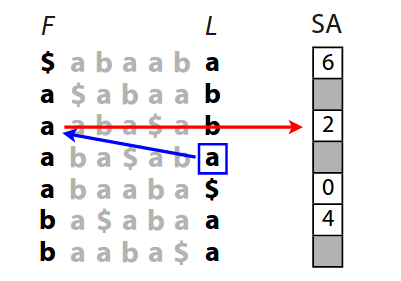
\includegraphics[width=.5\linewidth]{Figures/sa.png}
				\caption{SA sample example}
				\label{fig:sub1}
				\end{subfigure}%
				\begin{subfigure}{.5\textwidth}
					\centering
					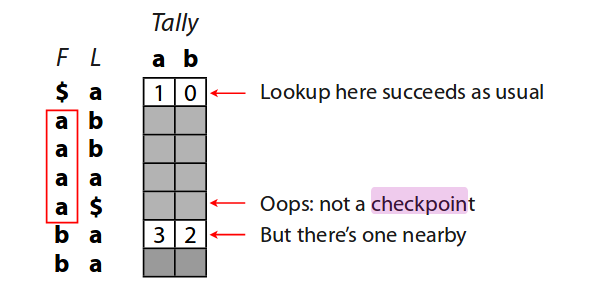
\includegraphics[width=.8\linewidth]{Figures/CHECKPOINT.png}
					\caption{Checkpoint example}
					\label{fig:sub2}
					\end{subfigure}
					\caption{Illustration of the two proposed improvement}
					\label{fig:test}
					\end{figure}
					
					Conclure
					
									

\section{Python Naive Implementation}

In order to get a better grasp of the concepts involved in the FM-Index implementation, a first one has been done in \textsl{Python}. The main advantage of this language is the syntax simplicity, allowing to focus on the algorithm and data-flow aspects of the string matching process while neglecting the data structures and global performances. \\

Good results have been reached using an adapted version of (CITER REPO), and this project has been used as a good basis for the less simple but way more precise \textsl{C++} implementation described in the next section. Below is a schema describing the software structure and execution flow.

[Poser un genre d'UML]

Using a terminal interface, the program is used as follow : 

[Mettre un screenshot]

\section{C++ Implementation}

All the software components of this project interacting with the board will be written in \textsl{C++}. This choice is based on legacy reasons (\textsl{REDS} environment) and conceptual reasons. The latter comes from the need to define a precise encoding of the \textsl{nucleotide reads} to be used on the FPGA system along with well defined and space-optimized data structures to store the \textsl{BWT} in the memory, the suffix array samples and the FM-Index checkpoints.

\subsection{Reads encoding and Data Structures}

\paragraph{Reads encoding}

Considering there are 4 different nucleotides within any DNA sequence, adding the uncalled base N type read and the "\$" equivalent character, we need to encode 6 symbols and thus need at least 3 bits. Therefore, it has been chose to use the following encoding : \\

\begin{minipage}[c]{0.35\textwidth}
\vspace*{6mm}
	\begin{tabular}{|c|l|}
	\hline
		Name & Encoding \\
		\hline 
		"\$" & 000 \\
		A & 010 \\
		C & 100 \\
		G & 101 \\
		T & 110 \\
		N & 111 \\
    \hline
	\end{tabular}
\end{minipage}
\begin{minipage}[t]{0.85\textwidth}
\vspace*{-30mm}
    \begin{minted}{c}
/* Type on 8 bits (only last 3 used) */
typedef unsigned char nucl_read; 
/* $ character */
static const nucl_read eos    = 0x00;	
static const nucl_read a_read = 0x02;
static const nucl_read c_read = 0x04;
static const nucl_read g_read = 0x05;
static const nucl_read t_read = 0x06;
static const nucl_read n_read = 0x07;
    \end{minted}
\begin{lstlisting}


\end{lstlisting}
\end{minipage}
\vspace*{3mm}

Dire un mot sur que quand meme voila c'est cool.
	

\paragraph{Data Structures}

Specific data structure will be needed in this program, not only to create the index and implement the whole algorithm, but also to be able to create files of a specific format containting the transform, the suffix array, etc. Those will then be used later with the hardware implementation of the index.

\begin{minipage}[t]{0.4\textwidth}
	\textbf{Checkpoint Entry -} \\
	\vspace{-5mm}
	\begin{minted}{c}   
typedef struct checkpoint_entry
{
    uint32_t eos_count = 0;
    uint32_t a_count   = 0;
    uint32_t c_count   = 0;
    uint32_t g_count   = 0;
    uint32_t t_count   = 0;
    uint32_t n_count   = 0;
	
} checkpoint_entry;
	\end{minted}
\end{minipage}
\hspace*{15mm}
\begin{minipage}[t]{0.5\textwidth}
		\textbf{BWT Class Attributes - }
\begin{minted}{c}
/* Last column = BWT(T) */
nucl_read * L;
/* First column of ordered SA */
nucl_read * F;	
/* First occurence array */
checkpoint_entry * occ;	
/* FM-Index samples */
checkpoint_entry * checkpoints; 
/* Sampled suffix array index's */
uint64_t * suffix_idx;	

	\end{minted}
	\textcolor{white}{.}\\

	
	
\end{minipage}
\vspace*{4mm}
Below is a schema describing the program structure and execution flow along with the files it produces from the FM-Index structures :

[Justifier les types, faire un UML ou quelque chose comme ca pour illustrer le fonctionnement]

Using a terminal interface, this program is used as follow :

[Poser un screenshot d'execution]


\section{Tests \& Validation}

[Benchmark pour C++ ??]